\textbf{Входные параметры:}

 x --- первая вещественная переменная;
 
 y --- вторая вещественная переменная.

\textbf{Возвращаемое значение:} 
 
Значение тестовой функции в точке $(x,y)$.

\textbf {Описание функции}

\begin{tabularwide}
\textbf{Идентификатор:} & MHL\_TestFunction\_Sombrero. \\
\textbf{Наименование:} & Функция Сомбреро. \\
\textbf{Тип:} & Задача вещественной оптимизации. \\
\end{tabularwide}

\textbf{Формула} (целевая функция):

\begin{equation}
\label{TestFunctions:eq:MHL_TestFunction_Sombrero}
f\left( \bar{x}\right) =\dfrac{1-{sin\left( \sqrt{\bar{x}_1^2+\bar{x}_2^2}\right)}^2 }{1+0.001\left(\bar{x}_1^2+\bar{x}_2^2 \right) }, \text{ где}
\end{equation}
\indent $\bar{x}\in X$, $\bar{x}_j\in \left[ Left_j; Right_j\right] $, $Left_j=-10$, $Right_j=10$, $j=\overline{1,n}$, $n=2$.

\begin{tabularwide}
\textbf{Обозначение:} &\specialcell{$\bar{x}$ --- вещественный вектор;\\$n = 2$ --- размерность вещественного вектора.}  \\
\textbf{Решаемая задача оптимизации:} & $\bar{x}_{max}= \arg \max_{\bar{x}\in X} f\left( \bar{x}\right)$.   \\
\textbf{Точка максимума:} & $\bar{x}_{max}={\left( 0, 0\right)}^\mathrm{T} $, то есть $\left(\bar{x}_{max} \right)_j=0$ ($j=\overline{1,n}$).    \\
\textbf{Максимум функции:} & $f\left(\bar{x}_{max} \right) =1$.   \\
\textbf{График:} & Рисунок \ref{TestFunctions:img:MHL_TestFunction_Sombreroe} нас \pageref{TestFunctions:img:MHL_TestFunction_Sombreroe} стр.   \\
\end{tabularwide}

\begin{figure} [h] 
  \center
  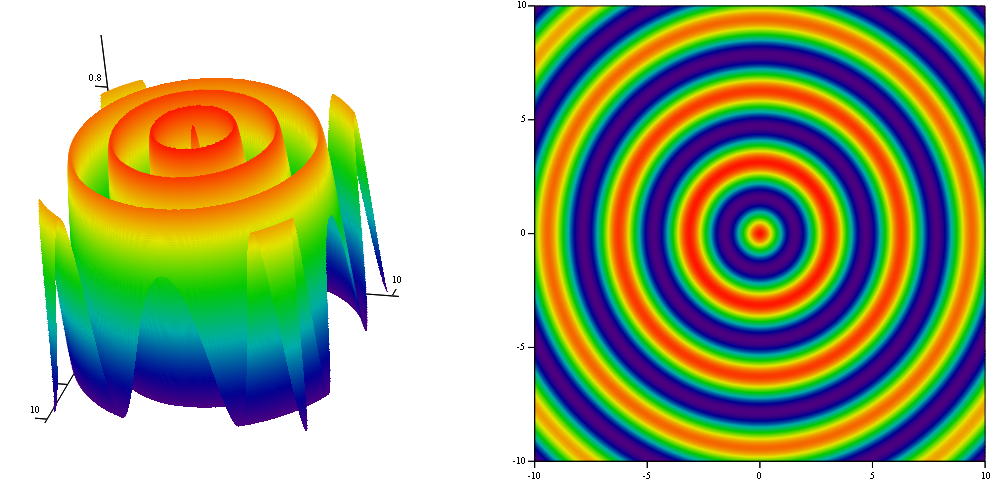
\includegraphics [scale=0.5] {MHL_TestFunction_Sombrero}
  \caption{Функция Сомбреро} 
  \label{TestFunctions:img:MHL_TestFunction_Sombreroe}  
\end{figure}

\textbf {Параметры для алгоритмов оптимизации}

\begin{tabularwide}
\textbf{Точность вычислений:} & $\varepsilon=0.05$. \\
\textbf{Число интервалов, на которые предполагается разбивать каждую компоненту вектора $\bar{x}$ в пределах своего изменения} (для алгоритмов дискретной оптимизации) : & $NumberOfParts_j=4095$ ($j=\overline{1,n}$). \\
\textbf{Для этого длина бинарной строки для $x_j$ координаты равна} (для алгоритмов бинарной оптимизации) : & $\left( k_2\right)_j=12$ ($j=\overline{1,n}$). \\
\end{tabularwide}

\textbf{Замечание:}  $NumberOfParts_j$ выбирается как минимальное число, удовлетворяющее соотношению:
\begin{equation*}
NumberOfParts_j=2^{\left( k_2\right)_j }-1\geq\dfrac{10\left( Right_j-Left_j\right) }{\varepsilon},\text{где } \left( k_2\right)_j \in \mathbb{N}, \left( j=\overline{1,n}\right).
\end{equation*}

\textbf {Основная задача и подзадачи}

\begin{tabularwide}
\textbf{Изменяемый параметр: } & $n$ --- размерность вещественного вектора. \\
\textbf{Значение в основной задаче:} & $n=2$.\\
\end{tabularwide}

\textbf {Нахождение ошибки оптимизации}

Пусть в результате работы алгоритма оптимизации за $N$ запусков мы нашли решения $\bar{x}_{submax}^k$ со значениями целевой функции $f\left( \bar{x}_{submax}^k\right) $ соответственно ($k=\overline{1,N}$). Используем три вида ошибок:

\textbf{Надёжность: }

\begin{equation*}
R = \dfrac{\sum_{k=1}^{N}S\left( \bar{x}_{submax}^k \right) }{N}, \text{ где}
\end{equation*}
\begin{equation*}
S\left( \bar{x}_{submax}^k \right)=\left\lbrace \begin{aligned} 1,& \text{ если } \left| \left( \bar{x}_{submax}^k \right)_j-\left( \bar{x}_{max} \right)_j\right|<\varepsilon, j=\overline{1,n};   \\ 0,& \text{ иначе}. \end{aligned}\right.
\end{equation*}

\textbf{Ошибка по входным параметрам:}

\begin{equation*}
E_x = \dfrac{\sum_{k=1}^{N} \left( \frac{\sqrt{\sum_{j=1}^{n}{\left( \left( \bar{x}_{submax}^k \right)_j-\left( \bar{x}_{max} \right)_j \right)}^2 }}{n} \right)  }{N}.
\end{equation*}

\textbf{Ошибка по значениям целевой функции: }

\begin{equation*}
E_f = \dfrac{\sum_{k=1}^{N} \left| f\left( \bar{x}_{submax}^k \right)-f\left( \bar{x}_{max} \right) \right|  }{N}.
\end{equation*}

\textbf {Свойства задачи}

\begin{tabularwide}
\textbf{Условной или безусловной оптимизации: } & Задача безусловной оптимизации. \\
\textbf{Одномерной или многомерной оптимизации: } & Многомерной: (двумерной). \\
\textbf{Функция унимодальная или многоэкстремальная: } & Функция многоэкстремальная. \\
\textbf{Функция стохастическая или нет: } & Функция не стохастическая. \\
\textbf{Особенности: } & Нет. \\
\end{tabularwide}